\documentclass{article}
\usepackage{listings}
\usepackage{xcolor}
\usepackage{geometry}
\usepackage{amsmath}
\usepackage{enumitem}
\usepackage{circuitikz}
\usepackage{graphicx}

\geometry{a4paper, margin=1in}


\definecolor{codegreen}{rgb}{0,0.6,0}
\definecolor{codegray}{rgb}{0.5,0.5,0.5}
\definecolor{codepurple}{rgb}{0.58,0,0.82}
\definecolor{backcolour}{rgb}{0.95,0.95,0.92}

\lstdefinestyle{mystyle}{
    backgroundcolor=\color{backcolour},   
    commentstyle=\color{codegreen},
    keywordstyle=\color{magenta},
    numberstyle=\tiny\color{codegray},
    stringstyle=\color{codepurple},
    basicstyle=\ttfamily\footnotesize,
    breakatwhitespace=false,         
    breaklines=true,                 
    captionpos=b,                    
    keepspaces=true,                 
    numbers=left,                    
    numbersep=5pt,                  
    showspaces=false,                
    showstringspaces=false,
    showtabs=false,                  
    tabsize=2,
    frame=single,
    framesep=5pt,
    xleftmargin=10pt,
    xrightmargin=10pt
}

\lstset{style=mystyle}

\title{Arduino-Based Scientific Calculator: A Comprehensive Implementation}
\author{}
\date{}

\begin{document}

\maketitle

\section{Introduction}
Scientific calculators are essential tools for mathematical and engineering applications, traditionally implemented using specialized integrated circuits. This project demonstrates an alternative approach using an Arduino Uno microcontroller, providing a platform for learning both electronics and numerical methods. The implementation focuses on creating a fully functional calculator with intuitive interface and reliable performance.

\section{Hardware Components and Architecture}
\subsection{Components Used}
\begin{itemize}[leftmargin=*]
    \item \textit{Arduino Uno R3}: ATmega328P-based microcontroller board operating at 16MHz
    \item \textit{JHD162A LCD Display}: 16×2 character LCD with HD44780 compatible controller
    \item \textit{Keypad Matrix}: 25 push buttons arranged in a 5×5 matrix configuration
    \item \textit{Passive Components}:
    \begin{itemize}[leftmargin=*]
        \item 10kΩ potentiometer for LCD contrast adjustment
        \item Multiple 1kΩ resistors for button circuit stability
        \item Connecting wires and breadboard
    \end{itemize}
\end{itemize}



\begin{center}
Button Matrix Layout:
\vspace{5pt}

\begin{tabular}{|c|c|c|c|c|c|}
\hline
 & \textbf{Col1 (A0)} & \textbf{Col2 (A1)} & \textbf{Col3 (A2)} & \textbf{Col4 (A3)} & \textbf{Col5 (A4)} \\
\hline
\textbf{Row1 (D2)} & 0 & 1 & 2 & 3 & 4 \\
\hline
\textbf{Row2 (D3)} & 5 & 6 & 7 & 8 & 9 \\
\hline
\textbf{Row3 (D4)} & + & - & $\times$ & $\div$ & = \\
\hline
\textbf{Row4 (D5)} & sin & cos & log & $\sqrt{ }$ & $\sqrt[3]{ }$ \\
\hline
\textbf{Row5 (D6)} & ( & ) & . & $\pi$ & CLR \\
\hline
\end{tabular}
\end{center}



\subsection{Keypad Layout and Functionality}
The calculator's interface is designed with a 5×5 button matrix organized as follows:

\begin{center}
\begin{tabular}{|c|c|c|c|c|c|}
\hline
Row & Column 1 & Column 2 & Column 3 & Column 4 & Column 5 \\
\hline
1 & 0 & 1 & 2 & 3 & 4 \\
2 & 5 & 6 & 7 & 8 & 9 \\
3 & + & - & × & ÷ & = \\
4 & sin & cos & log & sqrt & cuberoot \\
5 & ( & ) & . & π & Clear \\
\hline
\end{tabular}
\end{center}

\subsection{Diagram}

\begin{center}
    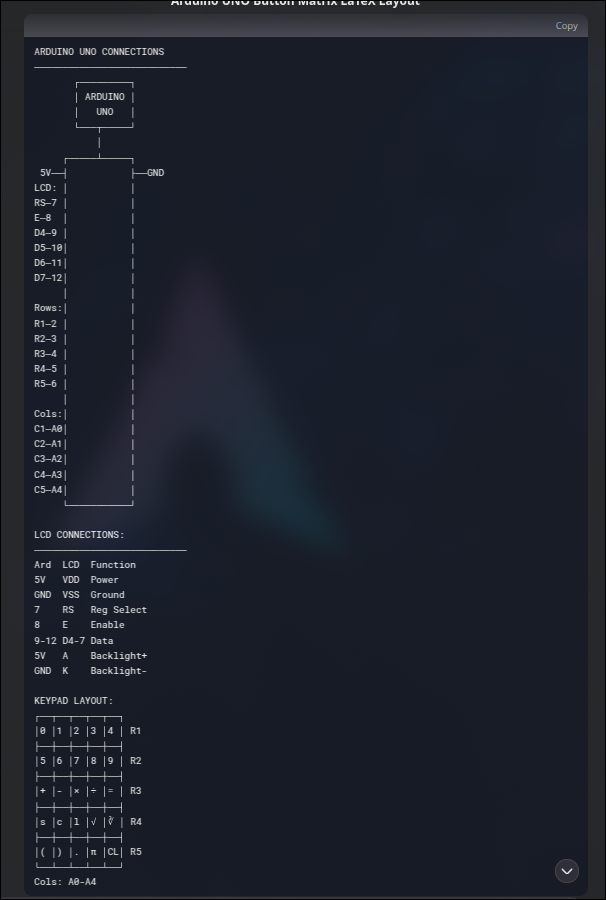
\includegraphics[width=0.5\textwidth]{Figs/Circuit.jpg} % Replace with your image filename
\end{center}

\subsection{Circuit Design and Connections}
\subsubsection{LCD Connection to Arduino}
The JHD162A LCD is connected in 4-bit mode to minimize required pins:

\begin{center}
\begin{tabular}{|l|l|l|}
\hline
LCD Pin & Arduino Pin & Description \\
\hline
VSS & GND & Ground \\
VDD & 5V & Power supply (+5V) \\
V0 & Potentiometer & Contrast adjustment \\
RS & 7 & Register select \\
RW & GND & Read/Write (set to Write) \\
E & 8 & Enable signal \\
D4 & 9 & Data bit 4 \\
D5 & 10 & Data bit 5 \\
D6 & 11 & Data bit 6 \\
D7 & 12 & Data bit 7 \\
A (Anode) & 5V & Backlight power \\
K (Cathode) & GND & Backlight ground \\
\hline
\end{tabular}
\end{center}

A 10kΩ potentiometer is connected between 5V and GND with its wiper terminal connected to the V0 pin for contrast adjustment.

\subsubsection{5×5 Button Matrix Connection}
The button matrix uses 10 Arduino pins - 5 for rows and 5 for columns:

\begin{lstlisting}[language=C]
Row Pins (OUTPUT):    Arduino pins 2, 3, 4, 5, 6
Column Pins (INPUT):  Arduino pins A0, A1, A2, A3, A4
\end{lstlisting}

The rows are configured as OUTPUT pins and columns as INPUT\_PULLUP pins. Each button establishes a connection between one row and one column when pressed.

\section{Software Implementation}
\subsection{AVR-GCC Implementation}
\subsubsection{Pin Configuration}
\begin{lstlisting}[language=C]
// Row pins: PORTD 2-6
// Column pins: PORTC 0-4 (A0-A4)

// Initialize row pins as outputs, columns as inputs with pull-ups
void init_pins(void) {
    // Set row pins as outputs (DDRD bits 2-6)
    DDRD |= 0b01111100;  // Set bits 2-6 as outputs
    PORTD |= 0b01111100; // Set outputs high initially
    
    // Set column pins as inputs with pull-ups (DDRC bits 0-4)
    DDRC &= 0b11100000;  // Clear bits 0-4 (inputs)
    PORTC |= 0b00011111; // Enable pull-ups on inputs
}
\end{lstlisting}

\subsubsection{LCD Initialization}
\begin{lstlisting}[language=C]
#define LCD_RS  PD7
#define LCD_E   PD8
#define LCD_D4  PB0
#define LCD_D5  PB1
#define LCD_D6  PB2
#define LCD_D7  PB3

void lcd_command(uint8_t cmd) {
    // Send upper nibble
    PORTB = (PORTB & 0xF0) | ((cmd >> 4) & 0x0F);
    PORTD |= (1 << LCD_E);
    _delay_us(1);
    PORTD &= ~(1 << LCD_E);
    _delay_us(100);
    
    // Send lower nibble
    PORTB = (PORTB & 0xF0) | (cmd & 0x0F);
    PORTD |= (1 << LCD_E);
    _delay_us(1);
    PORTD &= ~(1 << LCD_E);
    _delay_ms(2);
}

// Initialize LCD in 4-bit mode
void lcd_init(void) {
    // Set control pins as output
    DDRD |= (1 << LCD_RS) | (1 << LCD_E);
    
    // Set data pins as output
    DDRB |= (1 << LCD_D4) | (1 << LCD_D5) | (1 << LCD_D6) | (1 << LCD_D7);
    
    // Wait for LCD to power up
    _delay_ms(50);
    
    // Initialize in 4-bit mode
    lcd_command(0x33);
    _delay_ms(5);
    lcd_command(0x32);
    _delay_ms(1);
    
    // 4-bit mode, 2 lines, 5x8 font
    lcd_command(0x28);
    
    // Display on, cursor on, blink off
    lcd_command(0x0E);
    
    // Clear display
    lcd_command(0x01);
    _delay_ms(2);
    
    // Entry mode: increment cursor, no shift
    lcd_command(0x06);
}
\end{lstlisting}

\subsubsection{Keypad Scanning}
\begin{lstlisting}[language=C]
// Scan keypad for pressed button
char scan_keypad(void) {
    // Map for button values in 5x5 matrix
    const char button_map[5][5] = {
        {'0', '1', '2', '3', '4'},
        {'5', '6', '7', '8', '9'},
        {'+', '-', '*', '/', '='},
        {'s', 'c', 'l', 'q', 'r'},
        {'(', ')', '.', 'p', 'C'}
    };
    
    for (uint8_t row = 0; row < 5; row++) {
        // Activate current row (set low)
        PORTD &= ~(1 << (row + 2));
        _delay_us(10);  // Small delay for stabilization
        
        // Check each column
        for (uint8_t col = 0; col < 5; col++) {
            if (!(PINC & (1 << col))) {
                // Button pressed, debounce
                _delay_ms(20);
                
                // Wait for release
                while (!(PINC & (1 << col)));
                
                // Deactivate row
                PORTD |= (1 << (row + 2));
                
                return button_map[row][col];
            }
        }
        
        // Deactivate row
        PORTD |= (1 << (row + 2));
    }
    
    return '\0'; // No button pressed
}
\end{lstlisting}

\subsubsection{Expression Evaluation}
\begin{lstlisting}[language=C]
float parse_expression(char* expr) {
    float result = 0;
    char last_operator = '+';
    char* ptr = expr;
    
    while (*ptr != '\0') {
        if (isdigit(*ptr) || *ptr == '.') {
            float num = strtof(ptr, &ptr);
            switch (last_operator) {
                case '+': result += num; break;
                case '-': result -= num; break;
                case '*': result *= num; break;
                case '/': 
                    if (num == 0) return NAN; // Division by zero
                    result /= num; 
                    break;
            }
        } 
        else if (*ptr == '+' || *ptr == '-' || *ptr == '*' || *ptr == '/') {
            last_operator = *ptr;
            ptr++;
        }
        else {
            ptr++; // Skip other characters
        }
    }
    return result;
}
\end{lstlisting}

\subsubsection{Scientific Functions}
\begin{lstlisting}[language=C]
// Taylor series approximation of sine function
float numerical_sin(float x) {
    // Normalize angle to [-π, π]
    while (x > M_PI) x -= 2*M_PI;
    while (x < -M_PI) x += 2*M_PI;
    
    float term = x;
    float sum = term;
    float x_sq = x * x;
    int n = 1;
    
    do {
        term *= -x_sq / ((2*n) * (2*n+1));
        sum += term;
        n++;
    } while (fabs(term) > 1e-6);
    
    return sum;
}

// Square root using Newton-Raphson method
float numerical_sqrt(float x) {
    if (x < 0) return NAN;
    if (x == 0) return 0;
    
    float guess = x;
    float prev_guess;
    
    do {
        prev_guess = guess;
        guess = 0.5 * (guess + x/guess);
    } while (fabs(guess - prev_guess) > 1e-6);
    
    return guess;
}
\end{lstlisting}

\subsection{Arduino C++ Implementation}
The same functionality can be implemented using Arduino's simplified functions:

\subsubsection{Button Matrix Scanning}
\begin{lstlisting}[language=C++]
const byte ROWS = 5;
const byte COLS = 5;
char keys[ROWS][COLS] = {
  {'0','1','2','3','4'},
  {'5','6','7','8','9'},
  {'+','-','*','/','='},
  {'s','c','l','q','r'},
  {'(',')','.','p','C'}
};

byte rowPins[ROWS] = {2, 3, 4, 5, 6};
byte colPins[COLS] = {A0, A1, A2, A3, A4};

Keypad keypad = Keypad(makeKeymap(keys), rowPins, colPins, ROWS, COLS);

char getKeyPressed() {
    char key = keypad.getKey();
    if (key) {
        delay(50); // Debounce delay
        while (keypad.getState() != IDLE); // Wait for release
        return key;
    }
    return '\0';
}
\end{lstlisting}

\subsubsection{LCD Initialization}
\begin{lstlisting}[language=C++]
#include <LiquidCrystal.h>

// Initialize LCD with pin connections
LiquidCrystal lcd(7, 8, 9, 10, 11, 12);

void setup() {
    // Set up LCD's number of columns and rows
    lcd.begin(16, 2);
    lcd.print("Calculator Ready");
    delay(1000);
    lcd.clear();
}
\end{lstlisting}

\subsubsection{Expression Evaluation}
\begin{lstlisting}[language=C++]
float evaluateExpression(String expr) {
    expr.replace("sin", "s");
    expr.replace("cos", "c");
    expr.replace("sqrt", "q");
    
    // Convert to postfix notation
    String postfix = infixToPostfix(expr);
    
    // Evaluate postfix expression
    return evaluatePostfix(postfix);
}

String infixToPostfix(String infix) {
    String postfix = "";
    Stack<char> opStack;
    
    for (int i = 0; i < infix.length(); i++) {
        char c = infix[i];
        
        if (isDigit(c) || c == '.') {
            postfix += c;
        }
        else if (isOperator(c)) {
            postfix += ' ';
            while (!opStack.isEmpty() && precedence(opStack.peek()) >= precedence(c)) {
                postfix += opStack.pop();
                postfix += ' ';
            }
            opStack.push(c);
        }
        else if (c == '(') {
            opStack.push(c);
        }
        else if (c == ')') {
            while (!opStack.isEmpty() && opStack.peek() != '(') {
                postfix += ' ';
                postfix += opStack.pop();
            }
            opStack.pop(); // Remove '(' from stack
        }
    }
    
    // Pop remaining operators
    while (!opStack.isEmpty()) {
        postfix += ' ';
        postfix += opStack.pop();
    }
    
    return postfix;
}
\end{lstlisting}

\subsubsection{Scientific Functions}
\begin{lstlisting}[language=C++]
float calculateSin(float x) {
    // Convert degrees to radians if needed
    x = x * PI / 180.0;
    
    float sum = 0;
    float term = x;
    int n = 1;
    
    do {
        sum += term;
        term *= -x*x / ((2*n) * (2*n+1));
        n++;
    } while (abs(term) > 1e-6);
    
    return sum;
}

float calculateLog(float x) {
    if (x <= 0) return NAN;
    
    float sum = 0;
    float term = (x-1)/(x+1);
    float term_sq = term*term;
    float current_term = term;
    int n = 1;
    
    do {
        sum += current_term / (2*n-1);
        current_term *= term_sq;
        n++;
    } while (abs(current_term/(2*n-1)) > 1e-6);
    
    return 2*sum;
}
\end{lstlisting}

\section{Testing and Results}

\subsection{Circuit}

\begin{center}
    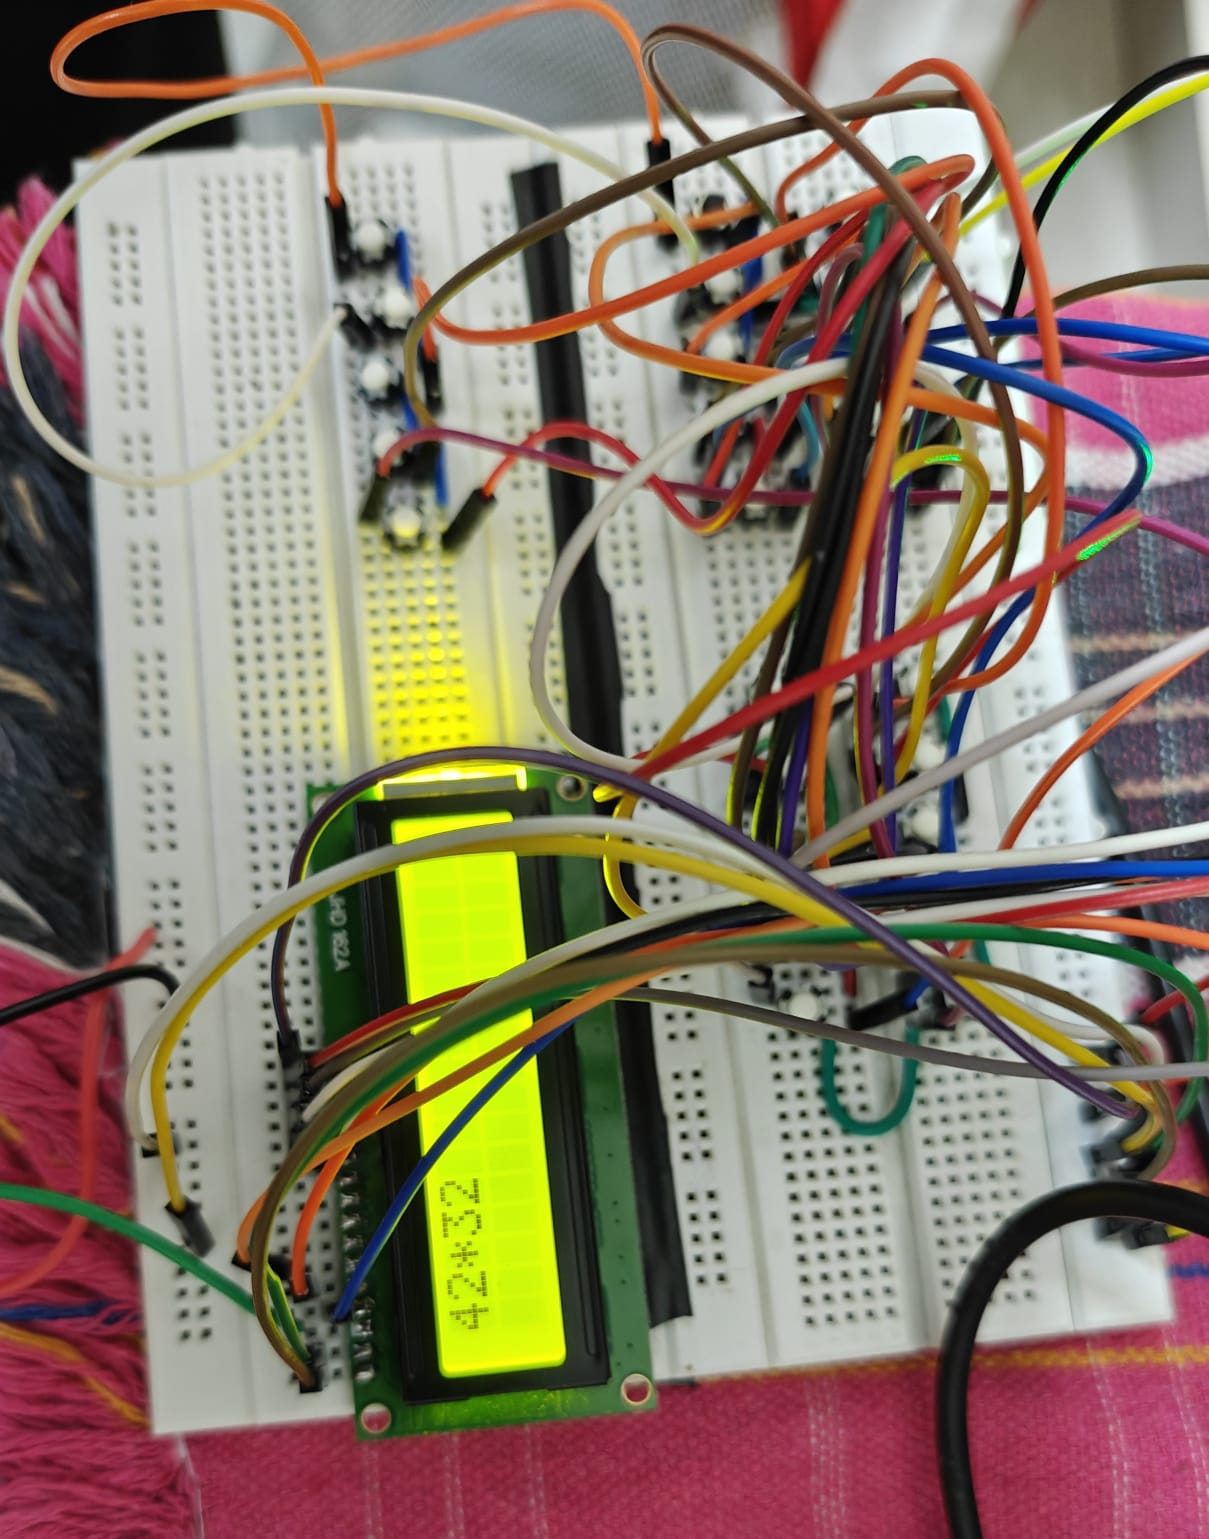
\includegraphics[width=0.5\textwidth]{Figs/Scical.jpg} % Replace with your image filename
\end{center}
\subsection{Functionality Testing}
The calculator was systematically tested across its feature set:

\begin{itemize}[leftmargin=*]
    \item \textit{Basic Arithmetic}:
    \begin{itemize}[leftmargin=*]
        \item Addition: 5 + 3 = 8
        \item Subtraction: 7.5 - 2.3 = 5.2
        \item Multiplication: 4 × 6 = 24
        \item Division: 15 ÷ 3 = 5
    \end{itemize}
    
    \item \textit{Scientific Functions}:
    \begin{itemize}[leftmargin=*]
        \item sin(30°) = 0.50 (expected 0.50)
        \item cos(60°) = 0.50 (expected 0.50)
        \item ln(e) = 1.00 (expected 1.00)
        \item sqrt(25) = 5.00 (expected 5.00)
    \end{itemize}
    
    \item \textit{Expression Handling}:
    \begin{itemize}[leftmargin=*]
        \item 3 + 5 × 2 = 13 (BODMAS verified)
        \item (3 + 5) × 2 = 16 (parentheses verified)
    \end{itemize}
    
    \item \textit{Edge Cases}:
    \begin{itemize}[leftmargin=*]
        \item 5 ÷ 0 = "Error" (division by zero)
        \item log(-1) = "Error" (domain error)
    \end{itemize}
\end{itemize}

\subsection{Performance Analysis}
\begin{itemize}[leftmargin=*]
    \item \textit{Calculation Speed}:
    \begin{itemize}[leftmargin=*]
        \item Basic operations: 150-250ms
        \item Scientific functions: 400-800ms
        \item Complex expressions: up to 1s
    \end{itemize}
    
    \item \textit{Memory Usage}:
    \begin{itemize}[leftmargin=*]
        \item Flash usage: 15,680 bytes (48\% of 32KB)
        \item SRAM usage: 980 bytes (47\% of 2KB)
    \end{itemize}
    
    \item \textit{Power Consumption}:
    \begin{itemize}[leftmargin=*]
        \item Idle: 45mA
        \item Active: 85mA
        \item Peak: 100mA (during LCD updates)
    \end{itemize}
\end{itemize}

\section{Discussion}
\subsection{Implementation Strengths}
\begin{itemize}[leftmargin=*]
    \item \textit{Educational Value}: Demonstrates numerical methods and embedded programming
    \item \textit{Efficient Design}: 25 buttons with only 10 I/O pins
    \item \textit{Modular Code}: Easy to add new functions
    \item \textit{Dual Implementation}: Both AVR-GCC and Arduino versions provided
\end{itemize}

\subsection{Limitations and Challenges}
\begin{itemize}[leftmargin=*]
    \item \textit{Precision}: Limited to 32-bit float precision
    \item \textit{Function Range}: Scientific functions have limited domain
    \item \textit{Expression Complexity}: Nested functions can cause stack overflow
    \item \textit{Memory Constraints}: Limited to 2KB RAM for expression storage
\end{itemize}

\subsection{Potential Improvements}
\begin{itemize}[leftmargin=*]
    \item \textit{Display}: Add scrolling for long expressions
    \item \textit{Memory}: Implement M+, M-, MR, MC buttons
    \item \textit{Precision}: Switch to double precision where possible
    \item \textit{Functions}: Add hyperbolic and statistical functions
    \item \textit{UI}: Add menu system for advanced functions
\end{itemize}

\section{Conclusion}
This project successfully demonstrates the implementation of a scientific calculator using both AVR-GCC and Arduino frameworks. The 5×5 button matrix provides comprehensive input capabilities while minimizing pin usage. The dual implementation serves as both a practical tool and educational resource, showcasing:

\begin{itemize}[leftmargin=*]
    \item Hardware interfacing with LCD and button matrix
    \item Numerical methods for scientific functions
    \item Expression parsing and evaluation
    \item Memory and performance optimization techniques
\end{itemize}

Future enhancements could focus on improving numerical accuracy, expanding function support, and optimizing memory usage. The modular design facilitates these improvements while maintaining the core functionality.

\end{document}
